\documentclass[11pt]{article}
\usepackage[margin=1.15in]{geometry}
\usepackage{amsmath,amssymb,amsthm}
\usepackage{booktabs}
\usepackage{graphicx}
\usepackage{microtype}
\usepackage[authoryear,round]{natbib}
\usepackage[colorlinks=true,linkcolor=black,citecolor=black,urlcolor=black]{hyperref}
\usepackage{setspace}
\onehalfspacing

\newtheorem{proposition}{Proposition}
\theoremstyle{definition}
\newtheorem{definition}{Definition}
\newcommand{\E}{\mathbb{E}}
\newcommand{\Cov}{\operatorname{Cov}}
\newcommand{\Var}{\operatorname{Var}}

\title{Where Covariance Comes From\\[4pt]
\large Log-Scale Slopes, Raw-Scale Slopes, and the Attribution of Correlation to the Asymptomatic}
\author{Flyxion\\Independent Researcher}
\date{October 2026}

\begin{document}
\maketitle

\begin{abstract}
\noindent
A recent analysis of symptom counts in a large adolescent cohort fits broken-stick regressions with a logarithmic link, finds that the rate-ratio slope relating one psychopathology dimension to another is several times larger at low symptom counts than at high counts, and concludes that covariation among dimensions is driven by the absence of symptoms and not by comorbidity. This essay examines what that pattern can and cannot establish. If the conditional mean of one count is linear in another on the raw scale, which is what a single shared continuous liability implies under standard count models, the log-scale slope declines with the predictor by construction, and a log-link broken-stick model will report a large pre-change slope and a small post-change slope with no special role for the asymptomatic. The same pattern also arises from a model in which an asymptomatic subgroup is the only source of association. The two models are separated by the raw-scale shape of the conditional mean, and the analysis reports a raw-scale check, in which the two slopes were almost identical, that points toward the first. The conclusion that covariance is mostly contributed by asymptomatic cases is further a statement about the decomposition of a covariance, which the analysis does not compute. For a linear conditional mean the decomposition is exact: a region contributes in proportion to its share of the predictor's variance. In a simulation with a single shared liability, the 79\% of cases below the change point contribute 28\% of the covariance. The statistical points are general and the empirical questions they raise are specific and answerable with the cohort data.
\end{abstract}

\section{The inference}

The analysis in question \citep{watts2026} applies Bayesian change-point regressions with a logarithmic link, and negative binomial errors, to symptom-count scores from four waves of a cohort of $11{,}868$ youths. For externalizing regressed on internalizing at the first wave, the change point lies at an internalizing count of $4.85$, the slope before it is $B_1=0.28$ (a $32\%$ increase in the expected externalizing count per symptom) and the slope after it is $B_2=0.07$ ($7\%$). The authors interpret the ratio of $4.6$ as showing that associations are strong at near-asymptomatic levels and weak at higher levels, and conclude that covariation among higher-order dimensions is driven by nomorbidity, which they define as the absence of symptoms and not the co-occurrence of disorders. They extend the interpretation to the p-factor, which they describe as appearing largely irrelevant to the clinical range.

Three separate inferences are packed into this. The first is descriptive: on the log scale, the slope declines with the predictor. The second is causal-structural: that decline means the covariance is contributed by asymptomatic cases and so is not evidence of comorbidity. The third is theoretical: a general factor is therefore uninformative at high severity. The first is a measurement the data can support. The second and third require more than the first provides, for two reasons that are mathematical and not empirical. The slope on a log scale is a different object from the covariance, and a declining log-scale slope is implied by simple models in which the association is the same at every level.

The paper deserves credit for several of its premises. Symptom data in community samples are skewed and zero-heavy, correlation-based methods depend on those distributional features, and reporting skewness and checking the linearity assumed by factor analysis is a good recommendation. The question here is the step from a declining rate ratio to a statement about where covariance comes from.

\section{A declining log slope is implied by a constant raw slope}
\label{sec:scale}

Let $X$ and $Y$ be counts and suppose $\E[Y\mid X]=a+bX$ with $a>0$, $b>0$. The log-link regression models $\log\E[Y\mid X]$. Its local slope is
\begin{equation}
\frac{d}{dX}\log\E[Y\mid X]=\frac{b}{a+bX},
\label{eq:logslope}
\end{equation}
which decreases in $X$. A fixed increase of $b$ in the expected count is a large relative increase when the expected count is small and a small relative increase when it is large. A broken-stick model with a single bend, fitted to this curve on the log scale, will report a steeper first segment and a flatter second one. No nonlinearity on the raw scale, and no special role for any subgroup, is involved.

The linear mean is not an arbitrary assumption. It is the implication of the standard model of a shared continuous liability under count noise.

\begin{proposition}
Let $\lambda\sim\mathrm{Gamma}(k,\beta)$ (shape $k$, rate $\beta$), $X\mid\lambda\sim\mathrm{Poisson}(c_1\lambda)$ and $Y\mid\lambda\sim\mathrm{Poisson}(c_2\lambda)$ independently given $\lambda$. Then
\begin{equation}
\E[Y\mid X]=\frac{c_2}{\beta+c_1}\,(k+X),
\end{equation}
which is linear in $X$ with slope $c_2/(\beta+c_1)$ at every level of $X$, and the log-scale slope is $1/(k+X)$.
\end{proposition}

\begin{proof}
By conjugacy $\lambda\mid X\sim\mathrm{Gamma}(k+X,\beta+c_1)$, so $\E[\lambda\mid X]=(k+X)/(\beta+c_1)$ and $\E[Y\mid X]=c_2\E[\lambda\mid X]$. The log slope is the derivative of $\log(k+X)$.
\end{proof}

With $k=0.7$, the log slope is $0.59$ at $X=1$ and $0.09$ at $X=10$. The values are of the same order as those reported for the cohort, $0.28$ and $0.07$. The proposition is not a fit to the data. It shows that a single shared dimension, the structure that the p-factor interpretation proposes, produces the reported qualitative pattern exactly, and with comparable magnitudes, when the data are analyzed on the log scale.

The analysis reports a check that bears on this. In a Gaussian one-change-point model with identity link, regressing externalizing on internalizing, the pre- and post-change slopes were almost identical to each other and to the one-slope estimate. The authors cite this to show that a change-point model does not manufacture nonlinearity. It also shows that the conditional mean was approximately linear on the raw scale, which by \eqref{eq:logslope} is precisely the case in which the log-scale slopes must differ. The authors set the Gaussian models aside because the error distribution is far from normal, which affects the standard errors and the likelihood comparison. It does not affect what a least-squares slope estimates, which is the best linear approximation to the conditional mean, and with robust standard errors the comparison is available. The result as reported is one pair at one wave. Whether it holds across the pairs and waves in the tables is an empirical question that the supplementary material can settle.

\section{A slope ratio is not a share of covariance}

The statement that covariance is mostly contributed by asymptomatic cases is a decomposition claim. It can be checked directly. For any partition of the sample by $X$,
\begin{equation}
\Cov(X,Y)=\sum_g p_g\,\E[(X-\mu_X)(Y-\mu_Y)\mid g],
\end{equation}
and for a linear conditional mean the regional contribution has a closed form.

\begin{proposition}
If $\E[Y\mid X]=a+bX$, the covariance contributed by a region $R$ of the predictor is $b\sum_{x\in R}p(x)(x-\mu_X)^2$, so its share of $\Cov(X,Y)$ equals its share of $\Var(X)$.
\end{proposition}

\begin{proof}
Summing $p(x)(x-\mu_X)(\E[Y\mid x]-\mu_Y)$ over $R$ and using $\E[Y\mid x]-\mu_Y=b(x-\mu_X)$ gives the stated expression.
\end{proof}

A skewed predictor concentrates its variance in the upper tail, since contributions are squared deviations from a mean that lies above the mode. A large group of cases near zero contributes little variance and so, for a linear mean, little covariance, however many of them there are. A claim that covariation is driven by asymptomatic cases therefore needs the regional decomposition and not a comparison of slopes, and the decomposition can differ in direction from the slope comparison. It is an easy quantity to report.

The slope ratio is also computed on a relative scale. The absolute slope at level $x$ is $\E[Y\mid x](e^{B}-1)$, so a relative slope of $7\%$ at a high expected count can exceed a relative slope of $32\%$ at a low one. With the reported rate ratios the absolute slope after the change point is the larger whenever the expected externalizing count there is more than about $4.5$ times its value before the change point. The reported tables give percentages and not the fitted intercepts, so the implied absolute slopes cannot be computed from them. The comparison would be immediate from the posterior draws.

\section{Two models, one pattern}

Two data-generating models, with sample size $11{,}868$ as in the cohort, make the logic concrete. They are illustrations and not fits, and the parameters are chosen to give plausible marginals.

\paragraph{Model A, one shared liability.} Each case has a shared Gamma component (shape $0.7$) and two specific components (shape $0.3$ each), all with rate~1. Internalizing is Poisson with mean $4.5\times(\text{shared}+\text{specific}_1)$ and externalizing is Poisson with mean $5.5\times(\text{shared}+\text{specific}_2)$. There is no asymptomatic subgroup in the construction. Cases with low counts are simply cases with low liability.

\paragraph{Model B, an asymptomatic subgroup.} A fraction $75\%$ of cases have no symptoms on either dimension. The remainder have independent negative binomial counts (size 1, means $18$ and $22$). The association is entirely a consequence of the asymptomatic subgroup.

For each model, one-change-point regressions with segments fitted by maximum likelihood (change point chosen by profile likelihood over integer values; Poisson quasi-likelihood with log link and a Gaussian identity-link version) were fitted to 30 simulated samples. Table~\ref{tab:fits} gives the averages.

\begin{table}[h]
\centering
\caption{Averages over 30 simulated samples of $N=11{,}868$. Log-link fits are Poisson quasi-likelihood. ``Covariance share'' is the fraction of the sample covariance contributed by cases below the fitted change point.}
\label{tab:fits}
\small
\begin{tabular}{lcc}
\toprule
 & Model A (shared liability) & Model B (asymptomatic subgroup) \\
\midrule
Pearson correlation & 0.59 & 0.42 \\
Change point (log link) & 7.8 & 2.0 \\
Log slopes, before / after & 0.162 / 0.048 & 4.06 / 0.00 \\
Rate-ratio increase, before / after & 18\% / 5\% & 5700\% / 0\% \\
Identity-link slopes, before / after & 0.689 / 0.704 & 21.7 / 0.002 \\
Share of cases below change point & 79\% & 78\% \\
Covariance share from those cases & 28\% & 23\% \\
\bottomrule
\end{tabular}
\end{table}

In Model A the log-link fit reports a pre-change slope $3.4$ times the post-change slope, close to the ratios reported for the cohort, while the identity-link slopes are $0.689$ and $0.704$ and the $79\%$ of cases below the change point contribute $28\%$ of the covariance. In Model B the log-link pattern is also steep-then-flat, but the identity-link slopes differ by four orders of magnitude. The two models therefore cannot be distinguished by the sign of the log-scale slope change, which both produce, and are distinguished at once by the raw-scale shape of $\E[Y\mid X]$ (Figure~\ref{fig:nomorb}, left).

\begin{figure}[h]
\centering
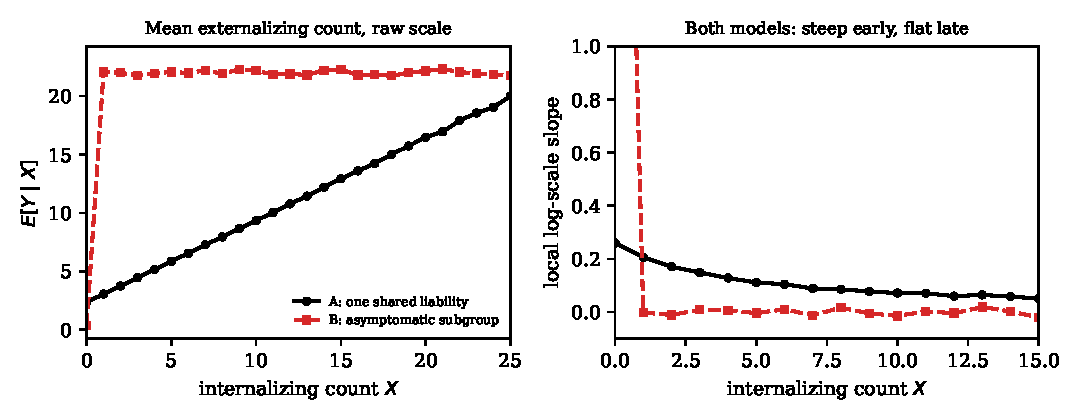
\includegraphics[width=\textwidth]{fig_nomorb.pdf}
\caption{Left: $\E[Y\mid X]$ in the two models on the raw scale, from $3\times10^{6}$ simulated cases. A is a line; B is a step. Right: the local slope of $\log\E[Y\mid X]$. Both are steep at low counts and flat at high counts.}
\label{fig:nomorb}
\end{figure}

Model B is the structure the nomorbidity interpretation describes: association generated by a subgroup with no symptoms at all. Model A is the structure the p-factor interpretation describes: association generated by a continuous shared dimension. Both look the same on the log scale. The raw-scale conditional mean in the cohort, to the extent the reported Gaussian slopes describe it, is nearer to Model A.

\subsection*{Shared absence is the low end of a shared dimension}

The analogy offered in support, from ecology, is that double absences should not count as evidence that two species are related. That is a well-founded rule for presence data where an absence can mean the habitat is unsuitable for both. In Model A, the double zeros arise from the same cause as the associations among the positive counts: low liability on a shared dimension. A person with no symptoms of either kind is the person at the bottom of the shared dimension, and calling that shared absence does not make it an alternative to the dimension. The two accounts are not exclusive, and the question of which one is supported is the question of raw-scale shape and of the decomposition, not of whether double zeros exist.

\section{What follows for the p-factor claim}

A decline in the log-scale slope does not show that a general dimension is irrelevant at high severity. For a linear mean, the expected change in externalizing per internalizing symptom is the same at every level, here $0.69$ and $0.70$. What does fall at higher levels is the correlation within a restricted range, since correlation is a ratio and the variance of the predictor and the count noise change across regions. An analysis that reports declining correlation or declining relative slopes at higher levels is compatible with a general dimension that affects all levels equally.

The paper meets the Berkson-type objection, that conditioning on high severity attenuates association, by noting that its change points sit at low counts. That answer addresses restriction by region. It does not address the choice of scale, which is the matter of Section~\ref{sec:scale}.

\section{Checks that would separate the accounts}

The analysis uses a rich cohort and the following checks require no new data.
\begin{enumerate}
\item Report identity-link slopes with robust standard errors for every pair and wave in the tables, and the raw-scale conditional mean as a binned plot with intervals. A constant raw slope favors the shared-liability reading; a step favors the subgroup reading.
\item Report implied absolute slopes $\E[Y\mid x](e^{B}-1)$ before and after each change point from the posterior draws, beside the relative ones.
\item Report the decomposition of the covariance and the correlation by region of the predictor, with intervals, so that the share contributed by cases below the change point is stated directly.
\item Fit a shared-liability count model matched to the observed marginals and apply the same change-point procedure. If it reproduces the reported pre- and post-change slopes, the pattern does not discriminate. If it does not, the pattern carries information.
\item Fit a mixture with an explicit asymptomatic class and compare its predictions with the raw-scale curve and the covariance decomposition.
\end{enumerate}
The negative binomial model's preference over the Gaussian one in model comparison concerns the error distribution as much as the mean function, so it does not by itself bear on the shape of the mean. Whether the supplementary material already contains any of these quantities was not examined; only the published main text was used here.

\section{Conclusion}

The measured fact, a larger rate-ratio slope at low counts, is reproduced by a model in which a single shared dimension drives association at every level, with the same raw slope throughout. It is therefore not evidence that the asymptomatic cases generate the covariance. The claim that they do is a decomposition claim, and for a linear mean the decomposition is controlled by the predictor's variance, which a skewed distribution places in the tail. The statistical lesson is general to count data analyzed with a logarithmic link: a slope on the log scale is a statement about relative change, and relative change declines with the level of the outcome even when absolute change does not.

\begin{thebibliography}{9}
\bibitem[Watts et al.(2026)]{watts2026} Watts, A.~L., Rosen, A.~F.~G., Greene, A.~L., King, K.~M., Meyer, F.~A.~C., Trull, T.~J., Sher, K.~J., Joyner, K.~J. (2026). Covariation among higher-order psychopathology dimensions is driven by nomorbidity and not comorbidity. \emph{Nature Mental Health}. doi:10.1038/s44220-026-00727-0.
\end{thebibliography}

\end{document}
